\setchapterpreamble[u]{\margintoc}
\chapter{Approach}
\labch{Approach}

%%%%%%%%%%%%%%%%%%%%%%%%%%%%%%%%%%%%%%%%%%%%%%%%%%%%%%%%%%%%%%%%%%%%%%%%%%%%%%%
%%%%%%%%%%%%%%%%%%% Motivation %%%%%%%%%%%%%%%%%%%%%%%%%%%%%%%%%%%%%%%%%%%%%%%%
%%%%%%%%%%%%%%%%%%%%%%%%%%%%%%%%%%%%%%%%%%%%%%%%%%%%%%%%%%%%%%%%%%%%%%%%%%%%%%%

\section{Motivation}
\labsec{motivation}

\todo{two stage approach be Ha and Schmidhuber 'world model'}

The basic approach of this work can be split into two steps:
\begin{enumerate}
    \item A differentiable renderer which can generate images of brush strokes from a parameter representation.
    \item An optimization procedure that iteratively approximates an image through brush strokes representations.
\end{enumerate}

The two step approach can be motivated by comparing the optimization procedure to the
actual process of painting an image.
An artist will most likely not pick single color particles to then place them on
the canvas.
Instead, the artist uses a brush or other utilities (see Pollock or others) to place
more paint with a single action.
\todo{image that shows different types of paint and tools etc.}
This of course limits the control over each individual drop of paint but maintains
enough control to still create very delicate details in paintings.
This trade-off varies for different brush sizes and for this reason an artist must
choose the brush size depending on the content.

An example would be the painting of a uniformly colored sky.
By using a large brush size the artist can cover a lot of canvas in relatively little
time as well as keep the color well distributed over the canvas because the brush
will spread color more or less evenly over its footprint.
On the other hand, if one were to draw a sky with the smallest brush available,
not only would it take forever to paint, it would also be hard to keep the paint
evenly distributed over multiple strokes.

Now, translating this onto the given problem of recreating/approximating an image
through brush strokes, it would mean to limit the process to only use what we would
describe as brush strokes. \todo{reformualte this}

An equivalent example would be the game of Tangram.

\begin{marginfigure}
    \includegraphics{tangram}
    \caption[]{An Example of Tangram.}
    \labfig{tangram}
\end{marginfigure}

Tangram is a Chinese puzzle game that has the objective of replicating a given silhouette
only with a set of 7 unique shapes.
The shapes may not overlay or be cut or anything.
Quite similarly, the objective for an optimizer is to replicate an image by only
using brush strokes.

\begin{marginfigure}
    \includegraphics{genetic_starry_night}
    \caption[]{Starry Night approximated by a genetic algorithm using only circles. \url{https://effyfan.com/2018/03/02/w6-van-gogh-flowfield/}}
    \labfig{genetic}
\end{marginfigure}

This is a similar task to what genetic algorithms already can do and have done in
order to approximate images by other geometric shapes or even smaller photos (also 
known as the popular photo mosaic effect).
\paragraph{Genetic algorithms} follow a random sampling approach that 'evolves' like genomes do.
Basically starting with a random set of circles that are parameterized by their position,
radius and color; it then chooses the most successful samples and resamples again
in a region around these.
This process is repeated again and again, until a certain level of convergence is reached.

As well as this does work, it is very much computationally expensive as most samples
will not fit the image, thus searching for the tiny set fitting shapes requires
to evaluate all the bad shapes as well.
Since brush strokes have many more degrees of freedom and artworks usually consist
of upwards of a few thousand brush strokes this will not be applicable to this problem
until computational resources have become a few magnitudes more powerful.

\begin{figure}
    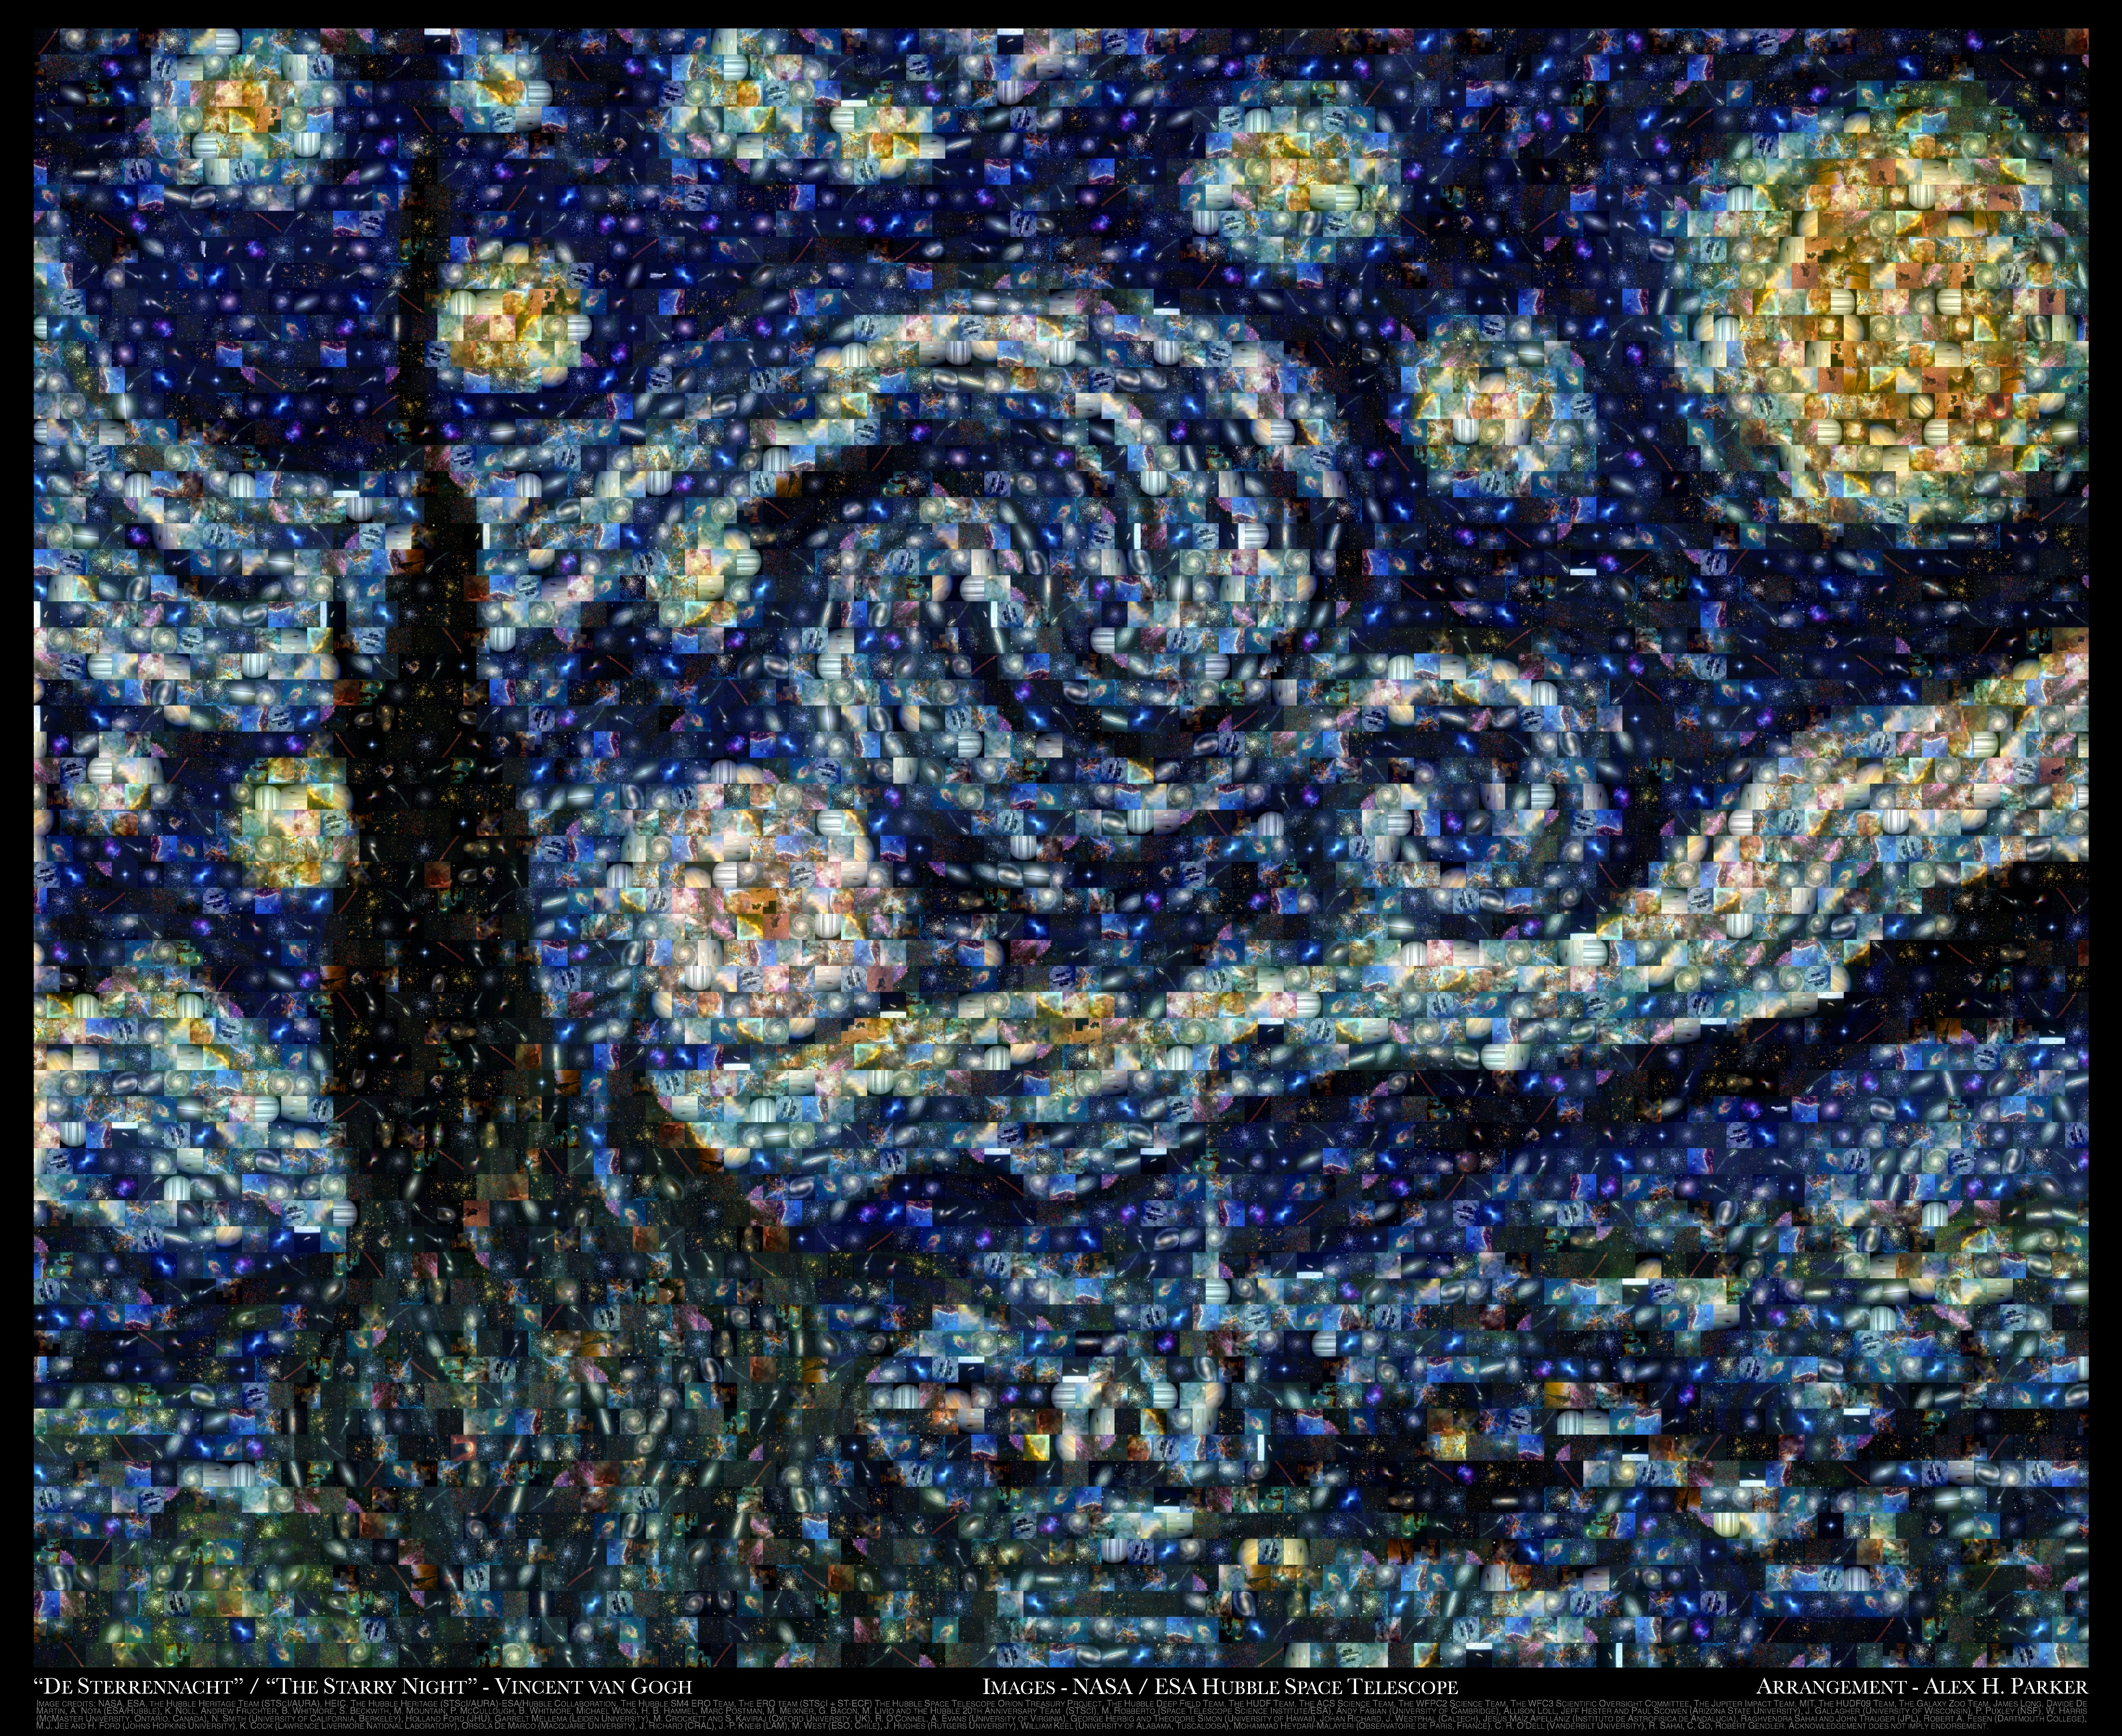
\includegraphics{photomosaic_starry_night}
    \caption[]{Photo mosaic of Starry Night using only images by the Hubble Space Telescope. \url{http://www.astro.uvic.ca/~alexhp/new/figures/starrynight_HST.001.jpg}}
    \labfig{photomosaic}
\end{figure}

This premise can be overcome, though, by using something that is known as as a differentiable
renderer.
\paragraph{Differentiable renderers} allow for the previously described task to be
feasible as random sampling is replaced by gradient descent.
A differentiable renderer is capable of creating shapes in the pixel domain by only
using differentiable operations.
Ordinary renderers do not have this property as they rely on faster operations that are
not differentiable as most renderers are not used in this context.
Also, creating a differentiable pipeline to render a circle from the tuple (position,
 radius, color) is a much harder task than calculation the shape of a circle beforehand
and then projecting the shape onto the pixels in an image and coloring them accordingly.
Nonetheless it is theoretically possible to create such a renderer.

Going back to the task of rendering brush strokes, it would be even harder to think
of a pipeline that uses only differentiable functions and is able to draw brush strokes
of a reasonable quality from a set of parameters.

This is where neural networks give an opportunity to avoid this problem.
Neural network are inherently differentiable and previous works have shown that
they are capable of high resolution and high quality conditional image generation.
One could easily think of a generator setup that takes as an input the parameters of
a brush stroke as well as some noise and then outputs an image of the according
brush stroke with possibly some variability in outline shape or other characteristics.

This principle was proposed by \cite{japanese neural renderer} as it facilitates
training of reinforcement learning based networks.

Inspired by this, the approach becomes more clear.
First, a differentiable renderer in form of a neural network is trained.
Then this renderer is used by an optimization procedure that uses gradient descent
to approximate an artwork as a input parameters batch of the renderer.

Both steps require some tricks to avoid pitfalls like computational limitation which
are outlined in the following two sections.

%%%%%%%%%%%%%%%%%%%%%%%%%%%%%%%%%%%%%%%%%%%%%%%%%%%%%%%%%%%%%%%%%%%%%%%%%%%%%%%
%%%%%%%%%%%%%%%%%%% Neural Renderer %%%%%%%%%%%%%%%%%%%%%%%%%%%%%%%%%%%%%%%%%%%
%%%%%%%%%%%%%%%%%%%%%%%%%%%%%%%%%%%%%%%%%%%%%%%%%%%%%%%%%%%%%%%%%%%%%%%%%%%%%%%

\section{Neural Renderer}
\labsec{NeuralRend}

The neural renderer is inspired by previous works (\todo{cite these works}) and 
is required to be differentiable and should be based on a rather simple architecture.
Especially since complicated architectures impose computational burdens and could
possibly distort the gradients for optimization.

\subsection{Data Set}
\labsubsec{dataset}

Unfortunately there is no data set available for this task which means that the data set
must be specifically created for this approach.

There are several sources for brush strokes that are evaluated in the following part.


\subsubsection{Brush Stroke Images}
\labsubsubsec{bsimages}

There are multiple sets of handrawn brush strokes available online.
Most notably there is a set of various well classified colors and brush styles created
by 'zolee' \todo{reference this} on the plattform \url{onlygfx.com}.
It cosists of approximately 1000 brush strokes that mostly follow rather straight
horizontal paths.
Brush strokes are mostly grouped by color and painting technique (oil, acrylic, watercolor...).
All images are in the PNG format and the area around the brush stroke was made 
transparent in a post-editing step.

This data set has the advantage that it consists of real world brush strokes that
were painted under presumably reproducible conditions.
On the other side, brush strokes are of mostly the same width throughout the data set
and also do not come with information which path the brush took or any other non-visual
information.
Also, the data is very sparse.
Many color shades are not represented which means that the generator would have to
'guess' them or simply would not be capable of rendering any brush strokes in this color.

It seems that this data set would be nice to replicate real world brush strokes
as images but limitations to the data make it unlikely that a generator could learn
a coherent representation from this.

\subsubsection{Painting Libraries}
\labsubsubsec{libmypaint}

The mentioned work of SPIRAL \todo{cite this} relies on opposite data to real world
images.
They used the painting library 'libmypaint' \cite{libmypaint} to generate brush strokes
from parameters in real time during training.

The obvious advantage of this and other painting libraries is the fact that one
can fully control the output through parameters.
This makes it much easier as the whole space of input parameters for the renderer
can be covered and avoids pitfalls like they were described in \ref{bsimages}.

Still, this data set falls short regarding the authenticity of rendered strokes.
Especially the inner area of the stroke shows a uniform color which is far from
what real brush strokes would look like.

This data set is better suited for our task than the given images are but will tend
to make all rendering look a bit 'cartoonish' or flat, which could in turn limit
convergence during the latter optimization process.

\subsubsection{Fluid Simulation}
\labsubsubsec{fluidpaint}

Fluid Paint \todo{cite website} is a project by \todo{name this guy} that uses simple
fluid dynamics to give artificial brush strokes a more plastic look.
It is implemented in JavaScript and OpenGL \todo{reference both}.

There is a C++ based version in the repository of SPIRAL which is also fitted with
python bindings by \todo{name that guy}.

Using these python bindings, it possible to generate brush strokes locally outside
of a web browser.

The quality and controllability of fluid paint falls right in between the two previously
mentioned datasets.
The generated brush strokes look distinctively better than those generated with 'libmypaint'
but still lack the quality of the real world images.
Concerning controllability, FluidPaint allows to control the path of the brush stroke
handle rather than the brush stroke itself.
This is a vast improvement over the images of 'zolee' but induces some offsets to
a given path as opposed to 'libmypaint'.

It seems that this is reasonable compromise between the previously mentioned data sets.
Although real time data generation in not possible with the library, it can be parallelized
to allow for the creation of large data sets in a reasonable time frame.

Even though this data set still has some weaknesses, it comes in as the probably best
choice for training a differentiable renderer because of the noted reasons.

\todo{add similar samples for all brush stroke methods.}

Other notable mentions are the painting programs \todo{these two weird software stuff things}
which allow for even more authentic brush strokes but lack a well documented interface
in order to generate a vast number of brush strokes.

\todo{talk about RGBA advantages}


\subsubsection{Brush Stroke Formalism}
\labsubsubsec{formalism}
With the means of data set production seized \todo{cut this joke}, what is left
is to formulate the parameters that define the brush strokes.
These parameters must quantify the following three properties of brush strokes:
\begin{itemize}
    \item color
    \item thickness
    \item path
\end{itemize}

The easiest of these three properties is quantifying the color.
Naturally, computer vision relies on the RGB format the defines color as a set of
three 8-Bit integer values between 0 and 255. 
As for path and thickness these two properties depend on the given coordinate system.
FluidPaint represents the canvas as a 2D plane in the $[0, 1]$ range, thus it makes
sense to follow the same representation.

Thickness thus becomes a value in $[0, 1]$  for each brush stroke, where 0 is and
infinitely small brush stroke and 1 is a brush stroke with the width of the canvas.
As both the edge cases do not make sense, the range is constrained to $[.03, .2]$
which includes only brush strokes that are visible and also do not cover the whole canvas.

Quantifying the path now is a little more tricky.
The fluid dynamics simulation that FluidPaint uses relies on internal time steps
at which the equations are evaluated and subsequently rendered.
At the same time each step allows only a linear motion of the brush handle between
positions $a$ and $b$.
This means that any curved paths must be split into linear/straight segments, that
should resemble a curved line.
As more steps mean longer simulation times and fewer steps mean edgy movement, a
value of 20 time steps per stroke is picked \todo{this is actually differernt as the steps depend on the lenght of the path. Look this up}.
This is equivalent to the number of steps that SPIRAL used in their implementation.

Another problem becomes how to express a curved path in numbers.
The easiest representation would be a sequence of points which make up the path of
interest.
This would give the highest versatility but at the same time introduce a noticeable
amount of parameters as each point consists of 2 coordinates rendering 40 values.
These values are also not independent but should follow are reasonable path as otherwise
the resulting brush stroke would look rather like a random walk than a believable
brush stroke.
Since works such as SPIRAL or Learning to Paint face a quite similar obstacle, their
solution should be applicable in this case as well.
Both works use so called 'Bezier curves' which parametrize curved paths by a limited
set of numbers.
\todo{image of bezier curve}

Bezier curves were invented in order to parametrize curved paths not through checkpoints
but analytical parametrizations for computer models.
They can be of different orders which allows them to follow more complicated paths
but in this case the simples form -- the first order -- is sufficient.
It defines a curve through its start and and point as well as a control point.
The curve is then defined as the path of a point over the time interval $[0, T]$.
First one connect the start and end points with the control point to get two lines
in return.
Along the lines on defines two points that move in a linear fashion along their lines
within the time interval $[0, T]$.
Then these two points are connected in the same way by a third line, which again
has a point moving along its direction over the span of $[0, T]$.
As the first two points that define the third line will move, the lines orientation
will change as well, thus translating the linear movement of the point into a complex
curved path.
The path that this point then takes in $[0, T]$ then defines the Bezier curve.
A first order Bezier curve will only bend into one direction or follow a straight path.
For higher orders the displayed process can be applied iteratively and allows for
more complex curves but as brush strokes usually follow a quite simple path and 
fewer parameters are preferred, Bezier curves of first order are chosen as parametrization.

Ultimately this gives 10 values that are sufficient to parametrize brush strokes
with certain constraints:
\begin{itemize}
    \item 3 two dimensional coordinates that define the Bezier curves (6 values).
    \item 1 thickness paramter.
    \item 3 values in RGB space.
\end{itemize}


\subsubsection{Data Constraints}
\labsubsubsec{constraints}

Given the parameters listed in section \ref{sssec:formalism}, the data still needs further
constraints to facilitate training of the generator even further.

Section \ref{sssec:fluidpaint} already hinted at the impracticality of online data generation.
A rough estimation by timing the rendering of 100.000 FluidPaint brush strokes reveals
that a dedicated CPU server is capable of generating 300 strokes per second when
using all of its resources.
\todo{experiment in appendix}
Keeping this in mind, a neural network with batch size 32 is limited to
$\approx 10$ terations per second which would mean a clear bottleneck.
Thus, it seems advisable to generate data beforehand with enough samples to cover
the data space sufficiently.
This will allow for much faster access to data, as individual data samples are relatively
small and can be stored in a binary data file such as HDF5.

Besides this constraint to the amount of data available, another set of constrains
will be introduced to reduce the data space to 'valid' brush strokes only.
'Valid' brush strokes will be defined as brush strokes which resemble real world
brush strokes to a certain degree.
This primarily concerns two relations within a brush stroke:
\begin{itemize}
    \item Its width-to-length ratio.
    \item Its curvature.
\end{itemize}

The width-to-length ratio will be restricted to brush strokes that are at least
two times as long as they are wide.
\begin{equation}
\norm{\vec{s} - \vec{e}} \overset{!}{\leq}  2 \times (\text{brush size}) \labeq{bs}
\end{equation}
Due to the simulation background of FluidPaint shorter brush strokes will show some
artifacts due to the bristles' length in the simulation which depends on the width
of the stroke.
Another reason for this, is the intended use case which will focus on van Gogh paintings.
As van Gogh did not practice pointillism most of his strokes have length to them,
which brings such a constraint in line with some characteristics of van Gogh's style.

The same argumentation can be done for the curvature:
Most brush strokes (especially those by van Gogh) have a certain 'flow' or 'smoothness'
to them, which can be described as by using strokes with large radii of their curvature
and without any corners in a strokes' path.
Thus data set will also be restricted to strokes which follow these descriptions.
In order to achieve this with random sampling in mind, a multivariate gaussian distribution
is placed between start point ($\vec{s}$) and end point ($\vec{e}$).
The two axes are rotated such that the short axis is in line with the vector
$\vec{a} = \vec{s} - \vec{e}$ while the other sits orthogonal.
Then both axes are scaled with $\norm{a}_2$ and also the handpicked values $\frac{1}{200}$
and $\frac{1}{25}$ for along $a$ and orthogonal to it, respectively.
Figure \ref{fig:datageneration} shows samples from this distribution for an exemplary
brush stroke.
\todo{draw figure in matplotlib or plotly or something}
This distribution is intended to follow that of brush strokes as they would appear
in the real world.
The majority of brush strokes will be straight or just slightly bent due to the maximum
of the PDF being at the center of $s$ and $e$.
Bent brush strokes will mostly be symmetric as the long axis of the multivariate gaussian
is orthogonal to $a$.
Still, there will be strokes that have their bent towards either end of the brush stroke
as well as some strokes with a high curvature.
The area of interest, though, will be densely populated as intended.
\begin{align}
    p(\vec{c}| \vec{s}, \vec{e}) & = \mathcal{N}(\mu, \Sigma) \labeq{checkpoint} \\
    \mu & = \frac{\vec{s} - \vec{e}}{2} + \vec{e} \\
    \Sigma & =
        \begin{pmatrix}
            \vec{a}_x & 0 \\
            0 & \vec{a}_y
        \end{pmatrix} \\
    \vec{a} & = \vec{s} - \vec{e}
\end{align}

The color of the brush strokes is not constrained as the color distribution of the
target data set is not known at this point. \todo{why not van gogh color distribution?}


%is this number of paramters enough, too much?

\subsubsection{Data Set Creation}
\labsubsubsec{creation}

The data set will be created with 100.000 samples that follow the constraints that
were presented in section \ref{sssec:constraints}.
As underlying distribution the uniform distribution is chosen as it allows a more
evenly coverage of the data space.

First, a set of start and end point as well as brush size is drawn and checked against
\eqref{eq:bs}.
If the constraint is not met, the set will be redrawn entirely.
In case the constraint is satisfied, a checkpoint is sampled according to \eqref{eq:checkpoint}.
If $\vec{c}$ lies outside the render window, the checkpoint will be resampled.
At last a color in form of an RGB value is sampled from a uniform distribution as well.

The resulting tuple of start, end and control point, brush size and RGB color is then
added to the data set.
Before rendering starts the values of $\vec{s}$, $\vec{e}$ and $\vec{c}$ are scaled
with the hand picked factor of $0.7$ to ensure the brush strokes are rendered completely
and not cut by the edge of the render window size.
At last the brush strokes are rendered according to the data set and added as well.
The render canvas size is 64x64 pixels.
\todo{why 64x64, explain this due to computational overhead, date requirements and training convergence}

As a last step, the data set is renormalized to the range $[-1, 1]$ for convenience
and to facilitate training as well.


\subsection{Architecture}
\labsubsec{arch}
The architecture of the brush stroke generator follows that of an inverse VGG network.
It is widely used and has shown in previous works that it should be capable of handling
this task.
\todo{check the details} The architecture consists of three dense layers at the beginning,
follow by an 2 times upsampling layer as well as three convolutional layers.
The same set of a 2 times upsampling layer and three convolutional layers is repeated
until the target size is reached.
After the last convolutional layer a tangens hyperbolicus function as applied, to
restrict the output to the $[-1, 1]$ range.
As part of the hyper-parameter search different tweaks to the architecture have been
tested:
\begin{itemize}
    \item An additional noise input at every layer with a size equal to that of the existing signal.
    \item Additional information about the position in the pixel grid in every layer, so called
        CoordConv \cite{coordconv}.
    \item Various combinations of activation and normalization functions.
\end{itemize}

\todo{network architectures as image}
The discriminator is designed after the same principles and resembles a VGG encoder
network
First three convolutional layers are applied, followed by a downsampling or pooling layer.
This is repeated until a target resolution of say 4x4 pixels is reached.
Then a set of three dense layers is applied to give one final prediction per sample.

\subsection{Training}
\labsubsec{train}
During training the L2 distance and the FID score were evaluated as metrics.
The FID score became necessary as the visual comparison of the generated samples
has proven difficult between different runs.
The L2 distance did not qualify as a sufficient metric for later training stages
as the stochastic nature of the brush strokes puts a threshold on how short the L2
distance can become.

To stabilize training further a two-time-step update rule was implemented.
\todo{write this down and look at the tricks that were used}

\subsection{Results}
\labsubsec{results}
\todo{pick some results and present whether they are any good}

%%%%%%%%%%%%%%%%%%%%%%%%%%%%%%%%%%%%%%%%%%%%%%%%%%%%%%%%%%%%%%%%%%%%%%%%%%%%%%%
%%%%%%%%%%%%%%%%%%% Stroke Approximation %%%%%%%%%%%%%%%%%%%%%%%%%%%%%%%%%%%%%%
%%%%%%%%%%%%%%%%%%%%%%%%%%%%%%%%%%%%%%%%%%%%%%%%%%%%%%%%%%%%%%%%%%%%%%%%%%%%%%%

\section{Stroke Approximation}
\labsec{strokeapprox}

\subsection{Dataset}
\labsubsec{dataset}
First off, for this section the data set will be presented.
This is due to the data defining some demands for the networks later on.
The data set for the optimization task should also meet a few requirements.

In order to be able to focus on the brush strokes in an image the data set should
consist of relatively high resolution images.
This becomes necessary as most brush strokes should fit into a 64x64 window any larger
strokes could not be approximated with a single renderer and thus would falsely be constructed
of multiple brush strokes.

This requires more information per image than simply the resolution as the scale
of the image plays into this requirement as well.
Ideally each image should be accompanied by its size as this allows to rescale all 
images accordingly, given that one knows how large a typical brush stroke is.

At last the painting's technique must be oil on canvas or similar techniques as this
is what the renderer has been trained for.

All these requirements on the data can be met by using data directly from the Van
Gogh Museum in Amsterdam that is freely available online.
Each high resolution image is categorized by its technique as well as the period
in which it was painted accompanied by information on the measurements of the image.

\subsection{Weapon of Choice}
The next stage of training takes the now pre-trained neural renderer and combines
it with the task of approximating brush strokes in images.
In theory the neural renderer should allow to gather gradients in parameter space
even though meaningful losses are calculated in image space, as explained in section
\ref{sec:motivation}.
There, it was outlined already that the weapon of choice will be an optimization
procedure that relies on the capabilities of the neural renderer.

But this is not the only possible approach to dissecting images into sets op parameters.
As explained in \ref{sec:PR} there exist a variety of approaches for this kind of
task.
Some of these promise fast generation of parameters from images which makes the 
optimization approach in this work seem like a step back at first.
The following section is dedicated to justifying the chosen approach by comparing
state of the art implementations of existing approaches.

The targeted task is to approximate the representation of an image with roughly
1MP by the means of $\approx 10.000$ brush strokes (see section \ref{ssec:motivation}).

\subsubsection{Genetic Algorithms}
\labsubsubsec{genalg}
Genetic algorithms are possibly the simplest approaches.
As it was laid out in sections \ref{sec:motivation} and \ref{sec:genetic}, genetic
algorithms use random sampling and previous best results to approximate fitting
solutions to the rendering problem which was described in section \ref{sec:renderproblem}.

Current state of the art solutions are capable of finding a solution in $\approx 1h$,
when searching for an approximation of a 1MP image with simple geometric shapes
like circles or triangles.
This accounts for roughly $1 \times 10^{9}$ sampling steps
This time frame varies depending on target shape density, target accuracy, sampling
runs per shape and degrees of freedom (with the latter requiring more sampling runs).

Looking back at seciton \ref{sec:renderer} each brush strokes has 10 degrees of freedom
with some inter-dependencies between them.
Also it is known that the obtained neural renderer is capable of generating $\approx
300 \frac{\text{images}}{s}$.
This means that rendering the same amount of sampled images will take:
$$
\frac{10^{9} \text{samples}}{300 \frac{\text{images}}{s}} \approx 3.33 \times 10^{6} s
\approx 926 h \approx 38.6 d
$$
Which is an impossible amount of time to spend \textbf{per image}.

At this point the number of samples has not been corrected for by the higher number of
degrees of freedom of this problem.

Ultimately this means that genetic algorithms are not an option for this task.

\subsubsection{Brush Stroke Extraction}
\labsubsubsec{bse}
Next in the line of approaches are algorithm based approaches that use standard
computer vision techniques to extract brush strokes from an image and parametrize them.

Besides texton based image characterization \cite{textons} and pure filter based
approaches \cite{filters} there have been approaches to extract brush strokes or
some of their characteristics \cite{brushstrokecharacteristics} \cite{brushstrokeextraction}.

The latter would pose a valid option for the main goal of this thesis if it were to
characterize brush strokes reliably.
Unfortunately the best existing techniques fail to detect brush strokes equally 
over the whole image but only identify the most significant ones (see figure \ref{fig brushstrokeextracted}).
Other approaches are only able to extract only few characteristics like the orientation
of a brush stroke, which proves insufficient as well.
\todo{show some of the extracted brush strokes}

\subsubsection{Stroke Based Rendering}
\labsubsubsec{sbr}
A different field that also uses algorithm to approximate an image through brush strokes
and also wants to achieve some stylization along the way is Stroke Based Rendering
or Painterly Rendering.
While early works relied on interactive approaches, later publications then were able
to fully automate this process.
Judging from tests by the authors themselves such an approach would take between \todo{this number}
and \todo{this number} hours per image to fully render it this way.
As figures \ref{fig:sbr1} and \ref{fig:sbr2} show, these approaches obtain similar
results to genetic algorithms and tend to draw and image from a coarse scale to a finer scale
instead of locally coherent.

At last these approaches were not intended to be used to obtain brush strokes from
a painting but rather focus on stylizing images.
This renders such an approach unfit for the goal of this thesis as well.

\subsubsection{Drawing Networks}
\labsubsubsec{drawingnetworks}
Lastly, drawing networks are the newest iteration of approaches in this field.
Beginning with \todo{which one was first?} there have been approaches the make use
of feed-forward or recurrent neural networks combined with either supervised training
or deep reinforcement learning.
The best results by these approaches are shown in figure \ref{fig:drawingnets}.

Noticeably, all of these images have a maximum resolution of 256 pixels along the
longer edge.
There have not been any approaches yet, which are able to go significantly beyond
this limitation.
Especially, the high computational costs of training recurrent neural networks seems
to be an obstacle when shooting for higher resolutions.
As it will be outlined in more detail in \ref{ssec:dataset} such resolutions can not
be deemed sufficient when looking at individual brush strokes.

This, also rules out drawing networks.

\subsubsection{Combined Approach}
\labsubsubsec{combinedapproach}

Even though there have been plenty of previous approaches to the task of extracting
brush strokes from images or to similar task like rendering images through brush strokes;
none of these quite meet all the requirements that have been posed for this task.
Namely, high resolution input images, brush stroke focussed rendering and/or retrieval,
limited resources and realistic depiction of brush strokes.

Even though brush stroke extraction seems to be most fit for the main asset of
this thesis, stroke based rendering and drawing networks both bring features into
the mix, that seem capable of making the task at hand more feasible.
Drawing networks for once introduced differentiable renderers as a tool to facilitate
training.
Stroke based renderers achieve a parametrization implicitly by focussing on replicating
the entire image instead of extracting brush stroke by brush stroke.

This can be combined into a unified approach that uses the differentiable renderer
and the objective of recreating an entire image.
The resulting approach does not use re-sampling like genetic algorithms do, but
can rely on gradient descent to converge to a solution significantly faster.

The limited capabilities of such a renderer would also guarantee that any approximation
is composed of only valid brush strokes instead of single pixels it would be the
case with normal generative models.

All in all such an approach fits best to the goal of this thesis as it will generate
an approximation of a target image that ideally resembles the target as closely as
possible while being limited to the use of brush strokes.



The decision of whether to use an optimization based approach is also linked to
another question: Whether to use a sequential or parallel placement of brush strokes.

As an example most drawing networks rely on a sequential approach as do some stroke
based renderers.
Intuitively it also makes sense to use a sequential approach as artists also place
their brush strokes sequentially on the canvas.
Yet there is a major difference in how existing computer vision based approaches
place their strokes compared to artists.
Due to the loss functions that are used when training drawing networks or stroke based
renderers the resulting images tend to be made up entirely of large canvas-filling
brush strokes which reduces the L2 loss very fast.

This is contrary to an artist which would maybe start with some sketches first but
then fills the canvas not with a brush that is roughly the size of the canvas -- as these
algorithms do -- but with a significantly smaller brush that requires many individual
strokes (often with some pattern) to fill large areas.
Thus, sequential approaches do actually differ significantly from how an artist would
paint.

In contrast to this parallel approaches which predict the whole painting in one step
are not wide spread due to the computational pitfalls that come with predicting
brush strokes for a whole painting at once compared to predicting only a few at a time.
Also, parallel approaches require to deal explicitly with the order in which brush
strokes should be placed on the canvas, as it will be explained in section \ref{sssec:order}.
Still, if one considers the optimization procedure instead of a policy network,
it becomes clear that the there are interactions between strokes that are locally
close.
An example would be one stroke in the foreground changing its path and revealing
the canvas beneath, then another stroke in the background should cover this up if
the color matches.

As usually artists plan their future brush strokes when painting the background
it would require a drawing network to plan far head which is impossible to do with
an optimization based approach.

Another argument for parallel optimization is the actual reliance on actual visual
proof for approximating brush strokes.
Sequential approaches will again an again cover up previous brush strokes until maybe
only a few pixels of the background brush stroke are visible.
Even if these few pixels match the target image well it will be a shot in the dark
whether this is really how the artist has drawn the background, which in return
introduces a great deal of noise to the result.
A parallel approach on the other hand should only place brush strokes where there
is visual evidence that there is a brush stroke and concentrate less on possible
background arrangements.

\subsubsection{Pitfalls of Feed-Forward Approaches}
\labsubsubsec{ffapproaches}

In the course of this thesis there were experiments targeting a feed forward approach
before ultimately tending toward the optimization based approach that is presented.

The main reason for this change in direction can be pinpointed to two problems that
emerged.
The computational burden that of a feed-forward approach can be approximated when
looking at existing feed-forward approaches of drawing networks.
Without compromising resolution and this images quality significantly, training
a network can hardly be realized.
Still it was possible to show a basic implementation of this for very simple data
like the cMNIST data set. \todo{margin explain cmnist} \todo{add image that were drawn by ff network}

Another problem that occurred was the placement of brush strokes on the canvas.
As artists are not bound to the same pixel grid as images are, they can place brush
strokes freely on the canvas.
More so, they can pack brush strokes densely in one area while distributing them
broadly in another.

As most neural networks in computer vision are CNNs, they are not able to allow for
a similar behaviour as they will always follow a grid layout of various resolutions.

Repeated experiments with either displaceable grid cells or stacked signals have proven
too complicated to manage for a convolutional network architecture and also seemed
to scale badly when implemented in fully convolutional manner.

Thus an optimization based approximation was chosen as it offers good approximations
at high resolutions with manageable computational overhead.

\subsection{Optimization Based Approach}
\labsubsec{opt}
Since the previous section \ref{ssec:ffapproaches} already specified why an optimization
based approach has been chosen over a feed forward or recurrent approach, this section
is meant to explain a little more about the optimization procedure itself.


\subsubsection{Rendering Layout}
\labsubsubsec{layout}
Fundamentally, the optimization procedure is inspired by stroke based rendering procedures.
Also, it could be compared to the style transfer approach by Gatys \etal \cite{gatys}, where, 
instead of pixels there a parameters optimized.
The difference to normal stroke based renderers, though, is the limited size of a
rendered brush stroke in this work's renderer.

This poses a significant challenge that might not be obvious at first.

Ideally the optimization procedure should be able to place strokes freely on canvas,
as this allows for an unbiased approximation.
Furthermore, this allows to allocate many small strokes in areas where the artist
placed many strokes as well and use fewer and wider strokes in other area during
the optimization procedure.
But due to various limitations which were explained in \ref{sec:NR}, the renderer
is not able to render single brush strokes in a 1MP frame.
Similar approaches only perform on relatively small canvas sizes, likely due to this
issue \todo{add ref}.

One work-around for this would be to dissect the target image into many smaller
patches and then run the optimization procedure on these individual patches.
This could be compared to a grid of renders where each grid cell is the center of
many renderings at the same time \todo{add figure to this}.
Right away, a major issue with this becomes obvious, which are the edges where the
grid cells are joined.

As a grid structure will almost always always differ from the inherent distribution
of brush strokes in an image, grid edges will more often than not, separate brush
strokes between two grid cells.
A simple solution to this problem is going from a stacked grid structure to an overlapping
grid. \todo{graphics!!!!!}

This hides obvious edges between render windows as every edge coincides with the center
of a different render window.
It is easily realized by choosing a lattice vector size smaller than the render window's
dimensions.

Still, this kind of initialization requires a very even distribution of brush strokes
with only small dislocations at each point in the lattice.
As this is not the case and stroke densities will vary locally, the grid layout is prone
to lead to enforcing a grid-like layout of strokes were there isn't any.
Mainly due to the inability of the grid to account for local changes in density and
the following propagation of error.
This would start with a single region of high density strokes in the vicinity of one
grid cell which would ideally result in a narrow stroke to achieve high accuracy.
Neighboring cells then have to shift their strokes towards the center of that grid cell
to account for the free space that is not covered by the narrow brush strokes.
This shift must then be accounted for by the next neighboring cells and so on, which
will cause all strokes in a raw or column to shift towards this one spot with a high
stroke density.

Now, a painting usually has many such high density areas which would require the
optimization procedure to balance the shift that is caused by these areas.
As a result the strokes are likely to not shift at all as shifting will equal out
for many such areas of high density.
Subsequently, an area of high stroke density will be not have enough strokes available
in its local region and thus will be covered up by a single broad stroke as this minimizes
the L2 loss.

The core of the problem is the previously imposed lattice structure that propagates
local density shifts along its principle axis.

One possible solution to this is getting rid of the lattice structure and replacing
it with a more random structure that also covers the image sufficiently.
This can be accomplished by using \textbf{super-pixels} \cite{superpixels}.
Super pixels come from an earlier era of computer vision and are often used in image
segmentation tasks (\cite{img segmentation with SP}) but super-pixels are also
a popular starting point for brush stroke extraction algorithms \cite{brushs stroke extraction}.

Basically, super-pixels are disjoint groups of pixels in an image that would usually
combine pixels with similar colors in a local region.
Straight away, it is obvious why this is interesting for brush stroke extraction.
In theory the distribution of super-pixels will not follow a grid-layout as the previous
approach and the location of super-pixels should relate to the given color distribution
in the image.
It is easy to imagine that the location of the super-pixel centers would be a good prior
of locations of render windows as well.
Also, as the colors of pixels inside a super-pixel should be similar, one can use
the mean color of a super-pixel as an initialization for the color of the brush stroke.

Ultimately, a super-pixel segmentation will be used to infer positions for render
windows as well as the color initialization of each strokes.

\subsubsection{Rendering Order}
\labsubsubsec{order}
Another problem that will come up during the optimization procedure is the order
in which strokes are rendered.
Real world brush strokes are also subject to the same issue as later brush strokes
will always be placed on top of earlier brush strokes, with no way of changing this
(see section \ref{sssec:combinedapproach}).

As the optimization based approach relies on parallel optimization of brush strokes,
it must be decided which strokes are in the foreground and which are in the background.
Otherwise, as this would randomly change, edges in the image might be obstructed
and optimization could oscillate between solutions where different strokes lie in
the foreground.
It could also lead to brush strokes not overlapping but covering disjoint areas.
All of these outcomes would be unfavorable as it tends to produce worse results
in the end.

The solution which is presented in this thesis is an additional parameter that describes
a brush stroke's accuracy.
The accuracy is defined as the L2 distance of each stroke's pixel to the corresponding
pixel in the target image multiplied by this each pixel's alpha value.
This removes any pixels which are of no interest from the loss and focusses only
on the rendered pixels.
\begin{align}
    \text{accuracy} = 1 - \frac{1}{N} \sum_{p \in \text{pixels}} \norm{p - p'}_2^2 \text{ with } \vec{p} = \vec{p'} 
\end{align}
    \todo{improve this}

The resulting value describes how well the pixels of the rendered stroke match their
respective pixels in the target image.
Consequently, any brush stroke with a higher accuracy will be more faithful to the
target image than strokes with a lower accuracy.
Placing these brush strokes in the foreground should thus result in a smaller L2 loss
than the other way around.
Vice versa, brush strokes which connect two same colored areas will aggregate a lower
accuracy as the brush stroke is compared at the intersection as well.
A rendered brush stroke which fits to the foreground brush stroke will not be affected by
such a penalty thus getting a higher accuracy and laying on top of the other brush
stroke.

Notably, the accuracy should not be included in the brush stroke's loss, as this
would prohibit background strokes from covering larger areas and result in behaviour
that is similar to non-overlapping issue previously described.
Thus, the accuracy of each stroke will be calculated as it is rendered.


\subsubsection{Initilization}
\labsubsubsec{init}

The following section will focus on initialization details for all parameters of a
brush stroke, their position and the confidence value.

Besides the original 10 parameters of each brush stroke, which were explained in
section \ref{sssec:formalism}, the previous two section introduced an accuracy
parameter for ordering and two translation parameters which define the position
of the render window along each axis.
All of these parameters must be initialized before the optimization procedure starts.
Ideally, the initialization should not introduce any bias to the optimization process.
At the same time an initialization should facilitate training and accelerate convergence
in early stages of optimization.

Unfortunately, the placement of the render window will surely enforce a bias on the
optimization as hinted in section \ref{sssec:layout}.
There a super-pixel initialization was motivated and for the translation parameters
as well as the color of the brush strokes.
Subsequently, the translation parameter for each render window will be equal to the
position of the weighted mass center of its respective super-pixel.

The initial color will be taken from the mean color value over the super pixel.

The brush size will be initialized with the minimum possible value.
This will let brush strokes not overlap at the beginning of optimization.
Only when the brush strokes already roughly fit their local region they shall intersect
and be ordered by their accuracy.
Therefore, the initial accuracy will be 0 everywhere, as the accuracy is recalculated
after every optimization step.

Other patch parameter, notably $\vec{s}$, $\vec{e}$ and $\vec{c}$, will be initialised
using a narrow normal distribution with $\sigma = .1$ and values clipped to $[-1, 1]$.
This is done, as there is no prior information available on how the brush strokes
are oriented.
Instead, this approach relies on the optimization procedure to be minimally biased
by this initialization of the path variables.

\subsubsection{Partial Updates}
\labsubsubsec{partupdate}

One major problem that emerges when building an optimizer based on the information
provided up until now, is the limitations of GPU memory.
Even as it might not be obvious at first, the optimization procedure imposes a huge
requirement for memory on the graphics card.
This is mainly due to two parts of the training:

First, the number of brush strokes can easily become very large, if large enough
images are used as input.
As the render window size of 64x64 already suggests the brush strokes are relatively
small and mentioned in section \ref{sec:motivation}, a painting can consist of a
few thousand brush strokes.
This would equate to a batch size of a few thousand for the brush stroke renderer.
Tests have shown that on an NVIDIA GTX 2080 Ti with 12GB GDDR5 VRAM the maximum number
of brush strokes rendered in parallel is $\approx 256$.
Obviously this is one to two orders of magnitude smaller than what would be needed
to optimize all stroke in the painting in parallel.
Still, there is a way around this bottleneck, by optimizing the image not as a whole
but as smaller patches consisting of 256 brush strokes at a time, giving a partial
update routine.

Each patch comprises the 256 nearest render windows to a randomly sampled location
on the canvas.
These 256 brush strokes are then rendered from their parameters in order to obtain
a gradient later on.
Then the strokes are placed on the canvas or 'padded' and than blended or 'stitched'
after they were ordered according to their accuracy.
At last, the loss is calculated and backpropagated to update the parameters of the patch.

As this will not make a difference for any brush strokes at the center of the patch,
border brush strokes (those which do not solely neighbor brush strokes that are also
optimized) will be affected by this.
This is the reason why it makes sense to safe the rendered brush strokes for all
parameters at any time forming a \textbf{render image catalogue}.
Equally the collection of brush strokes that shall later compose the image shall
be called a \textbf{parameter catalogue}.
With the render image catalogue at hand, it is possible to use the previously rendered
brush strokes to render the image as whole with the newly rendered brush strokes
of the image patch embedded.

As this will cause the border strokes to be surrounded by other brush strokes to all
sides (even if not all of them are freshly rendered) the effect of the partial update
routine vanishes.

The other problem that will occur for very large input images, is that the stitching
of brush strokes itself takes up a huge mount of RAM.
Going into detail, each brush stroke must be placed on the virtual canvas individually, 
where the canvas' size is that of the input image.
This would equate to a couple thousand 1MP images being stored in RAM before they
are stitched to a single 1MP images.
As a single 1MP image carries roughly $1000 \times 1000 \times 4 \text{channels}
\times 8 Bit = 32 \times 10^{6} Bit = 4 \times 10^{6} Byte = 4 MB$ of information,
a few thousand of these will easily eat up the RAM of most graphics cards.

Luckily, the previous work-around for optimizing only 256 brush strokes will work
as well without rendering the full image at every step.
Since most brush strokes are not re-rendered anyway and thus will not be supplied with
a gradient, their main task is to regulate losses for edge strokes of the image patch.
As this does not need far away strokes but only those close the strokes that are
optimized, a ring of pre-rendered strokes around the re-rendered patch will suffice.

\todo{approximate the amount of brush strokes needed to surround the patch}
This allows to reduce the amount of involved brush strokes per optimization step
from a few thousand down to a couple hundred.
Besides allowing for the partial update routine to be performed at all, it also
should increase performance significantly compared to an approach that involves
all brush strokes at any time.

\subsection{Image Placing and Blending}
\labsubsec{composition}
As the update and optimization procedure has now been explained thoroughly, it is
now time to explain the process of placing and blending a rendered brush stroke a
bit further.

After each stroke has been rendered it needs to be placed according to the translation
parameters that were introduced in section \ref{sssec:layout}.
This requires dynamically placing each brush stroke inside zero-filled tensor.

By calculating the global position of each pixel in the rendered image individually,
it is possible to scatter the pixels of the original rendered image into the larger
zero-filled tensor and obtain a globally placed brush stroke.

What is more complicated though is the task of blending the resulting canvas-sized
renders together or stitching them.
Due to the canvas' alpha channel it is possible to blend only relevant information
while the rest of the image will be ignored.

As far as conventional alpha blending goes, two images are blended by multiplying
each pixel value with the alpha value of the top-layer image while the background
image is multiplied with the complement to the alpha value:
\begin{align}
    p_{x,y} = p^{\text{top}}_{x, y} \times \alpha^{top}_{x, y}
    + p^{\text{bottom}}_{x, y} \times (1 - \alpha^{top}_{x, y})
    \forall (x, y) \in \mathcal{D}(\text{image})
\end{align}
\todo{correct this equation and make it nicer}

For multiple layers this process can be repeated in various fashions, after the strokes
are ordered according to their accuracy.
Either one could start from the bottom and blend the two back-most strokes, followed
by the next third last strokes and so one, or one could start this process from
the front with the two strokes in the very front being blended at first, then the
stroke with the third highest accuracy \etc.

Both of the approaches would yield the same result but differ only in the order in
which they were blended.
Subsequently, both methods will have $(n-1)$ blending operations to compute per pixel.

By moving from the linear approaches to a tree-based approach this number will not
decrease any further.

What makes it possible to reduce this number, though, is blending the strokes in 
a content aware fashion.
As looking at figure \ref{fig:stroke_on_canvas} shows, the majority of pixels for
each padded brush stroke is non-informative, as the alpha value is zero.
This hints at possibility to turn the process of blending around and instead of merging
layers subsequently as a whole, merging all layers at the same time by picking relevant
layers for each pixel.
Then all non-zero layers are merged in the same way as ordinary alpha blending works
but with the number of layers being reduced and information inside a layer not being
coherent anymore.


The easiest way to accomplish this is to first find the maximum depth over all pixels,
where the depth $k$ is the number of layers where the alpha value is not zero.
\begin{align}
    k = \argmax_{p \in \text{pixels}} \sum_{i \in \# \text{layers}} \mathds{1}(\alpha_i > 0)
\end{align}

Then the top $k$ layer indices for each pixel are picked, which reduces the number
of blending operations from $(n-1)$ to $(k-1)$.
Importantly, the top $k$ indices should not be ordered by their alpha values but
remain in the order that was imposed by sorting according to the accuracy value.
Otherwise, the order will most certainly be mixed up and the pixel with the highest
alpha value will always lie on top instead of the pixel that belongs to the most
accurate brush stroke.
Especially as brush stroke renderings fade out towards their edges, this makes a
significant difference.


Another way of accelerating the process of alpha-blending is vectorizing the process
instead of iteratively applying the computations.
To achieve this it is necessary to construct a tensor with the following properties:

For $\tensor{I} \in [0, 1]^{H \times W \times 4} $ the image target, the shape will be defined
as $\mathcal{S}(\tensor{I}) = (H, W, 4)$.
Each alpha channel will have the values $\alpha^{hw} \in [0, 1]$ for $h = 0, ..., H$ and $w = 0, ..., W$.

The set of rendered and padded brush strokes $\tensor{J}$ will have the shape $(N, H, W, 4)$
with $N$ depicting the number of brush strokes that ought to be stitched simultaneously.

Now, looking at each individual pixel in $\tensor{J}$, which is described by $(z^{hw}_n, \alpha^{hw}_n)$
for $n = 1, ..., N$ and $z^{hw}_n \in [0, 1]^{3}$, $z^{hw}$ describes the RGB values
and $\alpha^{hw}$ the alpha-channel for a pixel at $(h, w)$.

A blending operation can then be defined by
\begin{align}
    z'^{hw} & = \tilde{\alpha}^{hw} \cdot z^{hw} \\
    \text{or} \\
    z'^{hw} & = \sum_{n=1}^N \tilde{\alpha}^{hw}_n  z^{hw}_n \\
\end{align}

with $z'^{hw}$ the resulting RGB values of the blended pixel and $\tilde{\alpha}^{hw}$
a vector that holds the merged alpha values for each pixel:
\begin{align}
    \tilde{\alpha}^{hw} & =
    \begin{pmatrix}
        \alpha^{hw}_1 & &\\
        \alpha^{hw}_2 & (1 - \alpha^{hw}_1) &\\
        \alpha^{hw}_3 & (1 - \alpha^{hw}_2) & (1 - \alpha^{hw}_1)\\
        \vdots & &\\
    \end{pmatrix}
    = \alpha^{hw} \odot 
    \begin{pmatrix}
        1  &\\
        (1 - \alpha^{hw}_1) &\\
        (1 - \alpha^{hw}_2) & (1 - \alpha^{hw}_1)\\
        \vdots &\\
    \end{pmatrix}
    \\
    \rightarrow  \tilde{\alpha}^{hw}_n & = \alpha^{hw}_n \prod^{n-1}_{i=1} (1 - \alpha^{hw}_i)
\end{align}

Where $\odot$ describes the element-wise product.

What is left, is to find a way to construct $\tilde{\alpha}^{hw}$. from $\alpha^{hw}$.

blablabbla






%TODO explain the notation for alpha values with indices and what they mean

\todo{explain the alpha blending matrix}





\subsubsection{Losses}
\labsubsubsec{losses}

\todo{explain different loss combinations for different tasks}


\subsection{Results}
\labsubsec{results}

